\documentclass[tikz,border=10pt]{standalone}
\usepackage{tikz}
\usetikzlibrary{shapes.geometric, arrows.meta, positioning, fit, backgrounds, decorations.pathreplacing}

\begin{document}
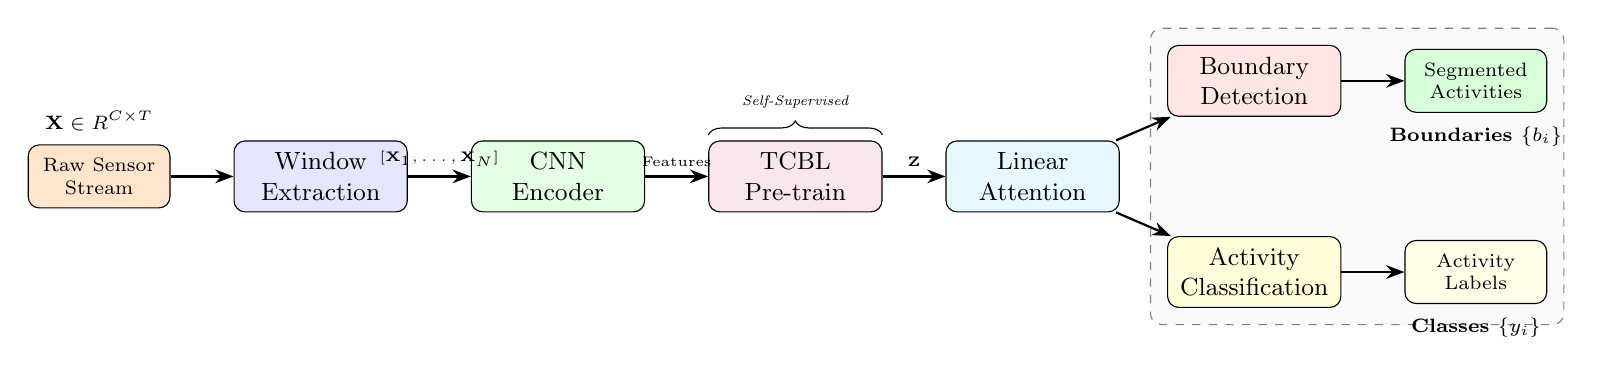
\begin{tikzpicture}[
    node distance=0.6cm and 0.8cm,
    block/.style={rectangle, draw, fill=blue!10, rounded corners, 
        minimum height=0.9cm, minimum width=2.2cm, align=center, font=\small},
    datablock/.style={rectangle, draw, fill=orange!15, rounded corners,
        minimum height=0.8cm, minimum width=1.8cm, align=center, font=\scriptsize},
    arrow/.style={-Stealth, thick},
    label/.style={font=\scriptsize\bfseries}
]

% Raw sensor stream
\node[datablock, fill=orange!20] (raw) {Raw Sensor\\Stream};

% Window extraction
\node[block, fill=blue!10, right=of raw] (window) {Window\\Extraction};

% CNN Feature Extraction
\node[block, fill=green!10, right=of window] (cnn) {CNN\\Encoder};

% TCBL Pre-training
\node[block, fill=purple!10, right=of cnn] (tcbl) {TCBL\\Pre-train};

% Linear Attention
\node[block, fill=cyan!10, right=of tcbl] (attn) {Linear\\Attention};

% Segmentation Head
\node[block, fill=red!10, above right=0.3cm and 0.6cm of attn] (seghead) {Boundary\\Detection};

% Classification Head
\node[block, fill=yellow!15, below right=0.3cm and 0.6cm of attn] (clshead) {Activity\\Classification};

% Segmented output
\node[datablock, fill=green!15, right=of seghead] (segs) {Segmented\\Activities};

% Classification output
\node[datablock, fill=yellow!10, right=of clshead] (labels) {Activity\\Labels};

% Arrows
\draw[arrow] (raw) -- (window);
\draw[arrow] (window) -- node[above, font=\tiny] {$[\mathbf{X}_1, \ldots, \mathbf{X}_N]$} (cnn);
\draw[arrow] (cnn) -- node[above, font=\tiny] {Features} (tcbl);
\draw[arrow] (tcbl) -- node[above, font=\tiny] {$\mathbf{Z}$} (attn);
\draw[arrow] (attn) -- (seghead);
\draw[arrow] (attn) -- (clshead);
\draw[arrow] (seghead) -- (segs);
\draw[arrow] (clshead) -- (labels);

% Labels
\node[label, above=0.05cm of raw] {$\mathbf{X} \in \mathbb{R}^{C \times T}$};
\node[label, below=0.05cm of segs] {Boundaries $\{b_i\}$};
\node[label, below=0.05cm of labels] {Classes $\{y_i\}$};

% Brace for self-supervised
\draw[decorate, decoration={brace, amplitude=5pt, raise=2pt}]
    (tcbl.north west) -- (tcbl.north east) 
    node[midway, above=8pt, font=\tiny\itshape] {Self-Supervised};

% Background for inference
\begin{scope}[on background layer]
    \node[fit=(seghead)(clshead)(segs)(labels), 
          draw=gray, dashed, rounded corners, 
          fill=gray!5, inner sep=6pt,
          label={[font=\tiny\itshape]above:Inference}] {};
\end{scope}

\end{tikzpicture}
\end{document}
